\documentclass[12pt]{article}
\usepackage{parskip}
\usepackage[T1]{fontenc}
\usepackage{graphicx}
\graphicspath{{images/}}
\usepackage{caption}
\usepackage{subcaption}
\usepackage{hyperref}

\title{A little Compiler}
\author{Joshua Leger, Fred Kneeland}
\date{Febuary 9, 2016}

\begin{document}
    \maketitle
    \begin{abstract}
	
		The goal of this project was to learn the fundamentals of compilation through the implementation of working compiler for the little language.  This project was done through Montana State University as the senior capstone project of the professional option for Computer Science.  	
	
    \end{abstract}
    \clearpage
    \tableofcontents
    \clearpage
    
    \section{Introduction}
		The goal of this project is to create a fully functioning compiler as the senior capstone project for the CS department at MSU.  The goal is that students will have a solid grasp on the mechanics and theory behind this integral component in most software development.  Over the course of several months a team of two seniors developed a complete compiler for the Little Language with a full functioning scanner, parser, symbol table and semantic routines.  Throughout the rest of the paper we will go over the various components of our compiler and how we developed each step as well as future work to improve the performance of the compiler.
		    
    \section{Background}
    	Compilers are a critical and foundation piece of computer science.  They are the tools that allowed for the abstraction of higher level languages, allowing far greater speed of development as well as rapid implementation of tedious optimizations.  As compilers are such critical tools in software development, learning both the theory and practical implementations behind them is an important aspect of any computer science education.  
    	Compilers are composed of several essential elements.  First there is a scanner.  A scanner is used to read in the code and to construct tokens that the compiler can understand.  The scanner is also used to find syntax errors.  Next there is a parser which takes all of the tokens generated by the scanner and creates a parse tree which is used to determine execution and to verify that the code actually forms a legal program.  Next there is a Symbol table which is used to generate and hold all of the variables and their values.  This symbol table is used in the final step of generating all of the Semantic routines in which the parse tree is converted to assembly code that can be run on a machine.  These four steps are used to take a high level language and convert it into something that can run on a machine either real or virtual. 
    	
    \section{Methods and Discussion}
    
    			This project was implemented in python and run from the command line.  A file was given to the program as an argument and the compiler would then parse that file.
    
    	\subsection{Scanner}
    			For the Scanner we utilized an open source python lexer by Dabeaz LLC.  We then used some regex statements to determine if an expression was valid and used that to validate the syntax and read in the expressions to be parsed. The following are the regular expressions used.

                First is the string literal:

                \begin{verbatim}
                    "[^"]*"
                \end{verbatim}

                This matches a quotation mark followed by 0 or more non quotation mark characters, ending in another quotation mark.

                Next are operators:

                \begin{verbatim}
                    <=|>=|:=|\+|-|\*|/|=|!=|<|>|\(|\)|;|,
                \end{verbatim}

                This was simply a large or statement, looking for each possible operator. Escape characters had to be used for +, *, (, and ). The <= and >= also had to come before < and > so it did not interpret <= as the < operator followed by the = operator.

                Float literals are defined as:

                \begin{verbatim}
                    [0-9]*\.[0-9]+
                \end{verbatim}

                Floats have 0 or more digits followed a period followed by 1 or more digits.

                Similarly, integer literals are defined as: 

                \begin{verbatim}
                    [0-9]+
                \end{verbatim}

                Integers are simply a list of 1 or more digits.

                Keywords and identifiers are defined with the same regular expression:

                \begin{verbatim}
                    [a-zA-Z][a-zA-Z0-9]*
                \end{verbatim}

                Identifiers are simply a letter followed by 0 or more letters and numbers. To identify keywords, a check on the string is run for equality to any of the keywords defined in the list named reserved defined at the top of the file.

                Finally, comments are defined as:

                \begin{verbatim}
                    --.*
                \end{verbatim}

                This matches a -- followed by the rest of the line. Instead of assigning a token to this, it is simply skipped over.

                Everything else is simply skipped over. This includes all whitespace.

                The order to search for tokens is string literal, float literal, int literal, operator, identifier, and keyword. Float has to be in front of int, but otherwise the order of checking does not matter.




    	\subsection{Parser}
    		For the parser we used the ply library.  With this library, yacc (Yet another Compiler Compiler) was used to do the manual labor of parsing through the tokens, once the grammar was provided.   In this stage of the project the formal definition of the Little Language was converted into a python grammar that the yacc parser could read in.  Using the Lexer created above, the parser was feed a string of tokens which it then evaluated as it built a parse tree.  
    		
    		We used the following structure to define a program: 
    		\begin{verbatim}
                    'statement : PROGRAM IDENTIFIER BEGIN pgm_body END'
           \end{verbatim}
           
           A program in the little language is composed of the keyword "PROGRAM" a name and then a code block in between the key words 'BEGIN' and 'END'
           
           The program body was defined as follows:
           \begin{verbatim}
                   '''pgm_body : decl func_decl'''
           \end{verbatim}
           
           Basically the program is divided into two sections.  The first is a list of global variables and the second section is all of the functions.
           
           the function list was defined as follows in such a way as to allow any number of functions including zero.
           
           \begin{verbatim}
           		'''func_decl : func_declaration func_decl
               	             | empty'''
            \end{verbatim}
            
            Similar to most c languages function declarations were composed of a return type, an indentifier, a list of parameters and a function body.
            
            \begin{verbatim}
                   '''func_declaration : FUNCTION any_type IDENTIFIER LEFTPAREN param_decl_list RIGHTPAREN BEGIN func_body END '''
           \end{verbatim}
           
           The paramater list is defined as a list of variable types and names separated by commas.
           
            \begin{verbatim}
                   '''param_decl_list : param_decl param_decl_tail
                                              | empty'''
           \end{verbatim}
           
			A param decl is where parameters name and type is specified.
			
			\begin{verbatim}
           '''param_decl : var_type IDENTIFIER'''
           \end{verbatim}
			            
           The param decl tail was used to ensure that the variables were seperated by Commas and that the list could be extended.
           
           \begin{verbatim}
                   '''param_decl_tail : COMMA param_decl param_decl_tail
					                           | empty'''
           \end{verbatim}
           
           The func body is very similar to the program body as it is composed of two pieces, variable declarations and statements.
           
           \begin{verbatim}
                   '''func_body : decl_func_var stmt_list'''
           \end{verbatim}
           
           Inside of stmt list is where most of the heavy lifting of the program takes place.  Statements include all of the operations, conditional statments and loops.
           
            \begin{verbatim}
                  '''stmt_list : stmt stmt_list
				                    | empty '''
				   '''stmt : base_stmt
             				   | if_stmt
		               	   | while_stmt'''
           \end{verbatim}
           
           Base Statements are used for all of the standard one line operations such as assigning values, or expressions, to variables, returning values, reading, and writing.
           \begin{verbatim}
                   '''base_stmt : assign_stmt
					                    | read_stmt
					                    | write_stmt
					                    | return_stmt'''
           \end{verbatim}
           
           Assignment statements are used for handling operations and various types of expressions.
           
           \begin{verbatim}
           		'''assign_stmt : assign_expr SEMICOLON'''
           		'''assign_expr : IDENTIFIER STRINGEQUALS expr'''
            \end{verbatim}		
           
			Expression statements allow for any combination of variable operators.  
			
			\begin{verbatim}
				"expr : expr_prefix factor"      
				'''expr_prefix : expr_prefix factor addop
                                   | empty'''
			\end{verbatim}	   
			
			Factors represent various kinds of values.  They can be variables, constants or function calls.
			
			\begin{verbatim}
				'''factor : factor_prefix postfix_expr'''
				'''factor_prefix : factor_prefix postfix_expr mulop
				                       | empty'''
				'''postfix_expr : primary
			                          | call_expr'''  
			    "call_expr : IDENTIFIER LEFTPAREN expr_list RIGHTPAREN "                                          
			\end{verbatim}	
			
			Statements can also be conditional statements.
			\begin{verbatim}
"if_stmt : IF LEFTPAREN cond RIGHTPAREN decl_block_var
stmt_list else_part ENDIF"
            \end{verbatim}	
           
            Additionally, statements can become loops.
            \begin{verbatim}
"while_stmt : WHILE LEFTPAREN cond RIGHTPAREN decl_block_var
stmt_list ENDWHILE"
            \end{verbatim}
           
    		
    		Overall the Little language is a very simple language with a few strict rules which significantly reduce complexity.  Each program has a program definition with a body that is composed of two sections.  The first section defines variables and the second is for functions.  The functions themselves have a very limited subset of options with conditional systems and only a while loop.  Therefore an unambiguous grammar for this language proved to be a relatively trivial task.  
    		

    	\subsection{Symbol Table}
    		Now that the compiler parses through the tokens the next step is to create a symbol table.  For this aspect of the project we created a couple of data structures.  First we had a variable object which would hold information about a specific variable including its name and value.  Additionally, we created a symbol table object.  This object had a parent, a list of children and a list of variables.  Furthermore, we also stored the current scope level.  Thus we could navigate up the scope list to find a declaration of a variable or we could add another scope as a child if we had a function or Block statement.  
    		This was accomplished by adding code to the parsing rules.  Under each rule that dealt with variables in the parser the current symbol table had to be updated.  Because of the way that the symbol tables were created we started with a global symbol table.  We also had a variable that pointed to the current symbol table.  Then whenever there was a variable declaration it was added to the current symbol table.  In the same way when a new scope was encoutered it was added as a child of the current symbol table and the current symbol table was then updated to be the newly created table.  Then when the scope was exited the current symbol table variable was updated to be its parent. 
    		
    		The main difficulty for constructing the symbol table was from ply.  When parsing the leaves were executed first.  This meant that the parser would find a variable declaration before it knew what symbol table the declaration was suppose to be a part of.   To counteract this, temporary symbol tables were created and when the declaration of a function or Block statement was hit these were then appended to the correct symbol table.  The same was true of individual variables and in order to meet the requirement that variables appear in the proper order in the symbol table, variables needed logic about whether to be inserted at the beginning or end of the variable list in order to maintain their proper orientation relative to one another.

    	\subsection{Semantic Routines}
    		The goal of the semantic routines is to generate the assembly code for the program.
            It creates an intermediate representation and then converts that to the actual assembly required by the tiny simulator.
            The intermediate representation is a linked list of 3 address codes that is generated during parsing and utilizes the symbol table.
            The codes are:
            \begin{verbatim}
ADDI   OP1 OP2 RESULT
ADDF   OP1 OP2 RESULT
SUBI   OP1 OP2 RESULT
SUBF   OP1 OP2 RESULT
MULTI  OP1 OP2 RESULT
MULTF  OP1 OP2 RESULT
DIVI   OP1 OP2 RESULT
DIVF   OP1 OP2 RESULT
STOREI OP1     RESULT
STOREF OP1     RESULT
GTI    OP1 OP2 LABEL
GTF    OP1 OP2 LABEL
GEI    OP1 OP2 LABEL
GEF    OP1 OP2 LABEL
LTI    OP1 OP2 LABEL
LTF    OP1 OP2 LABEL
LEI    OP1 OP2 LABEL
LEF    OP1 OP2 LABEL
NEI    OP1 OP2 LABEL
NEF    OP1 OP2 LABEL
EQI    OP1 OP2 LABEL
EQF    OP1 OP2 LABEL
JUMP           LABEL
LABEL          STRING
READI          RESULT
READF          RESULT
WRITEI         RESULT
WRITEF         RESULT
            \end{verbatim}

            The codes were created and chained together throughout parsing, while keeping track of temporary variables and labels that the codes generated.
            For example, given the following piece of code:
            \begin{verbatim}
A := B + C * D
            \end{verbatim}
            The parser would first generate
            \begin{verbatim}
MULTI C D $T1
            \end{verbatim}
            It would store the MULTI command at the head of the linked list and return \$T1 up through the parser.
            Next the parser would generate
            \begin{verbatim}
ADDI B $T1 $T2
            \end{verbatim}
            It got passed the \$T1 variable for the second arguement and generates \$T2, passing it up again.
            Finally, it would generate
            \begin{verbatim}
STOREI $T2 A
            \end{verbatim}
            The final code for the line is a linked list of 3 lines,
            \begin{verbatim}
MULTI C D $T1
ADDI B $T1 $T2
STOREI $T2 A
            \end{verbatim}
            This list is then passed up higher and combined with other statements to create a linked list that is the full intermediate representation.

            Another example is the while loop.
            Take the following:
            \begin{verbatim}
i := 10;
WHILE (i != 0)
    i := i - 1;
ENDWHILE
            \end{verbatim}
            The parser would first generate
            \begin{verbatim}
STOREI 10 $T1
STOREI $T1 i
            \end{verbatim}
            It wold then generate the code for conditional statement inside the parentheses.
            \begin{verbatim}
STOREI 0 $T2
EQI i $T2 label1
            \end{verbatim}
            Next, it generates the code to execute inside the loop.
            \begin{verbatim}
STOREI 1 $T3
SUBI i $T3 $T4
STOREI $T4 i
            \end{verbatim}
            Finally, it combines all sections of the code with the neccessary jump and label statements.
            \begin{verbatim}
STOREI 10 $T4
STOREI $T4 i

LABEL label2 

STOREI 0 $T5
EQI i $T5 label1

STOREI 1 $T6
SUBI i $T6 $T7
STOREI $T7 i

JUMP label2 
LABEL label1
            \end{verbatim}
            Most of the parts are created whether it was part of a loop or not and the loop just combines them all.

            From there, it is a simple matter to convert all the 3 address codes to 2 address codes that the tiny simulator can run.
            For STORE, the conversion is
            \begin{verbatim}
STORE OP1 RESULT
================
move OP1 rx
move rx RESULT
            \end{verbatim}

            For READ and WRITE, the conversion is
            \begin{verbatim}
READ/WRITE RESULT
=================
sys read/write RESULT
            \end{verbatim}

            For ADD, SUB, MULT, and DIV, the conversion is
            \begin{verbatim}
ADD/SUB/MULT/DIV OP1 OP2 RESULT
===============================
move OP1 rx
add/sub/mult/div op2 rx
            \end{verbatim}

            For LABEL, the conversion is
            \begin{verbatim}
LABEL STRING
============
label STRING
            \end{verbatim}

            For JUMP, the conversion is
            \begin{verbatim}
JUMP LABEL
==========
jmp LABEL
            \end{verbatim}

            For GT, GE, LT, LE, NE, EQ, the conversion is
            \begin{verbatim}
GT/GE/LT/LE/NE/EQ OP1 OP2 LABEL
===============================
move OP2 rx
cmp OP1 rx
jgt/jge/jlt/jle/jne/jeq LABEL
            \end{verbatim}

    	\subsection{Full fledged Compiler}
            The main components of the compiler are the lexer and parser.
            First, the lexer runs through the code and generates symbols from the raw text.
            Next, the parser using the symbols to ensure correct syntax and generate the symbol table and intermediate code.
            Finally, the intermediate code is converted into tiny code, which is output and can be run.
            \begin{center}
                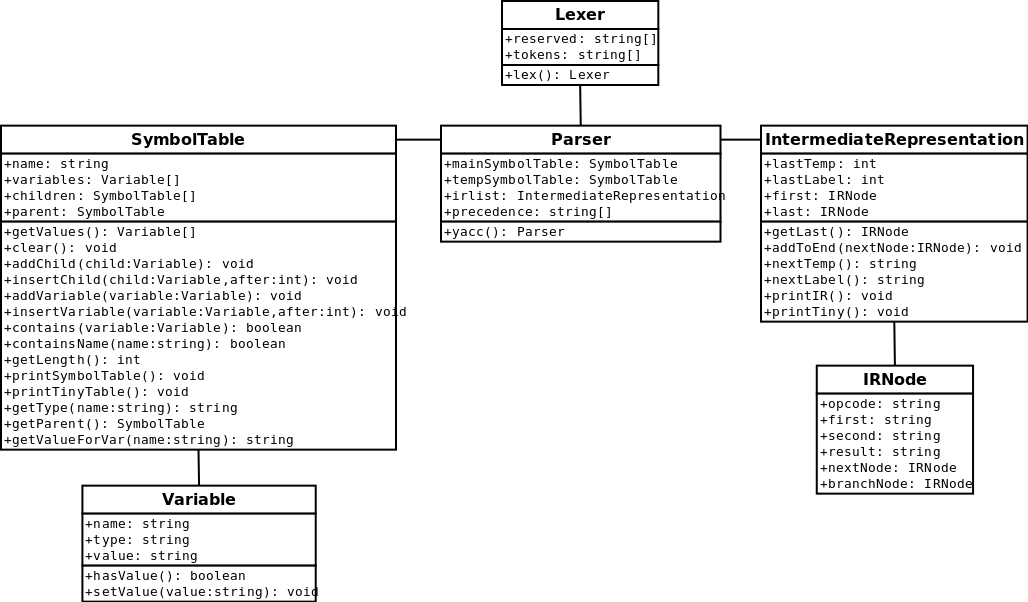
\includegraphics[width=\linewidth]{uml}
            \end{center}

    \section{Conclusion and future work}	
			While a fully functional compiler was working by the end of this project there are several body's of work remaining.  First was that no optimizations were made to the compiler.  If this compiler was going to be used in a real life production setting then this would be a serious issue of concern.  The first optimization that should be developed is CSE (common subexpression elimination) in order to minimize redundant operations.  Second, register allocation should be done in a more efficient manner.  In order to accomplish this the compiler should create a liveness tree for registers.  Then when a register is no longer being used it should "kill" it and use that register for other values in the rest of the program.  
			In addition to optimizations the next stage of development should include expanding the use of functions in the code.  Currenlty the semantic routines does not contain support for function declaration or calls other than the main function.  As any significant code base should be broken into multiple functions this is a critical piece of development before this compiler can be considered operational.
    
 \end{document}
